  \sectioncounter{3}
  \section{函数的概念及表示, 定义域与值域}

  \subsection{知识梳理}
  设有两个数集 $A$, $B$, 若对任意 $x\in A$, 按确定的对应法则 $f$, 
  有唯一的 $y\in B$ 与之对应, 则称 $y$ 是 $x$ 的\myindex{函数} (function), 
  记为 $y=f(x)$, 并把 $A$ 称为\myindex{定义域} (domain), 
  $B$ 称为\myindex{值域} (range). 
  定义域、对应法则和值域也称为\myemph{函数的三要素} (前两者决定了第三者).
  由定义, 函数是数集之间的映射, 不允许一对多, 但可以多对一 (如 $y=x^2$). 
  高中数学只考虑定义域和值域均为 $\mathbb{R}$ 或其子集的情形.
  
  函数的常见表示法有\myemph{列表法} (作图时常用), \myemph{图象法}, \myemph{解析法} (用具体式子表示对应法则).
  若函数 $f$ 在其定义域不同的部分有不同的表达式 (解析式), 则称其为\myindex{分段函数} (piecewise function). 有的分段函数也可用一个式子表示, 如
  \[f(x)=|x|=\begin{cases}x,& x\geqslant 0,\\ -x,& x<0.\end{cases}\]
  
  若无特殊说明, 通常认为函数的定义域是使函数表达式有意义的自变量取值范围, 
  此时的定义域也称为函数的\myemph{自然定义域}. 常见的函数自然定义域中, 需特别注意的有:
  \begin{align*}
    \dfrac1x\colon x\neq 0,\quad 
    & \quad\sqrt{x}\colon x\geqslant 0,
    \qquad \tan x\colon x\neq \frac\pi2+k\pi, k\in\mathbb{Z},\\
    a^0\colon a\neq 0,\quad 
    & \quad a^x,\ \log_a x\colon a>0 \text{ 且\ }a\neq 1,\ x>0.
  \end{align*}
  
  函数的值域一般可由函数的图象得到, 而图象又由其单调性决定. 
  求函数单调性的通用方法是考虑函数的导数的正负. 
  
  \lianxi
  \begin{exercise}
    若函数 $f(x)=x-x^2$,则 $f(x+1)-f(x)=$\,?
  \end{exercise}

  \beginsolution
    $f(x+1)=(x+1)-(x+1)^2=-x-x^2$, 则 $f(x+1)-f(x)=-2x$.
  \endsolution
  
  \begin{exercise}
    已知函数 $y=\begin{cases}
      x^2+1, &x\leqslant 0,\\
      -2x,   &x>0,
      \end{cases}$
    那么使函数值为 $5$ 的 $x$ 的值是\,?
  \end{exercise}

  \beginsolution
    当 $x>0$ 时, $y<0$, 则 $x\leqslant 0$ 且 $x^2+1=5$, 解得 $x=-2$.
  \endsolution
  
  \begin{exercise}
    函数 $f(x)=\sqrt{x-1}+\dfrac1{x+4}$ 的定义域为\,?
  \end{exercise}

  \beginsolution
    $x-1\geqslant 0$ 且 $x+4\neq 0$, 解得 $x\in[1,+\infty)$.
  \endsolution
  
  \begin{exercise}
    函数 $f(x)=\dfrac1{1-x}+ \log_3(3x-1)$ 的定义域为\,?
  \end{exercise}

  \beginsolution
    $1-x\neq 0$ 且 $3x-1>0$, 解得 $x\in\Big(\frac13,1\Big)\cup(1,+\infty)$.
  \endsolution
  
  \begin{exercise}
    函数 $y=x-x^2$ ($x\geqslant 0$) 的最大值为\,?
  \end{exercise}

  \beginsolution
    由函数图象知, $x=\frac12$ 时, $y=\frac14$ 为最大值.
  \endsolution
  
  \subsection{要点导学\quad 各个击破}
  \subsubsection{函数的三要素}
  \begin{example}
    下列各组函数中, 表示同一函数的是 $\underline{\qquad\qquad}$. (填序号.)

    $(1)\ f(x)=x-1$, $g(x)=\dfrac{x^2}{x}-1$;\qquad
    $(2)\ f(x)=|x|$, $g(x)=(\sqrt{x})^2$;

    $(3)\ f(x)=x$, $g(x)=\sqrt[3]{x^3}$;\qquad
    $(4)\ f(x)=2x$, $g(x)=\sqrt{4x^2}$.
  \end{example}

  \beginsolution
    (1) $f(x)$ 中 $x\in\mathbb{R}$, $g(x)$ 中 $x\neq 0$;
    (2) $f(x)$ 中 $x\in\mathbb{R}$, $g(x)$ 中 $x\geqslant 0$;
    (3) $g(x)=x=f(x)$; (4) $g(x)=2|x|\neq f(x)$, 故填 ``(3)''.
  \endsolution
  
  \lianxi
  \begin{exercise}[s]
    下列各组函数中, 表示相同函数的是 $\underline{\qquad}$. (填序号.)

    (1) $f(u)=\sqrt{\dfrac{1+u}{1-u}}$, $g(v)=\sqrt{\dfrac{1+v}{1-v}}$;

    (2) $f(x)=\sqrt{x^2}$, $g(x)=x$.
  \end{exercise}

  \beginsolution
    (1) $f(x)=g(x)$; (2) $f(x)=|x|\neq g(x)$, 故填 ``(1)''.
    \mymarginpar{只要两个函数的定义域和对应法则相同, 这两个函数就相同, 无需表示自变量的字母相同.}
  \endsolution
  
  \subsubsection{求函数的解析式}
  \begin{example}
    (1) 已知 $f\Big(\dfrac1x\Big)= x^2+5x$, 求 $f(x)$ 的解析式;

    (2) 设 $f(x)$ 是一次函数, 且 $f\bigl(f(x)\bigr)=4x+3$, 
      求 $f(x)$.
  \end{example}

  \beginsolution
    (1) 设 $t=\frac1x$, 则 $t\neq 0$, $x=\frac1t$, 所以 \[f(t)=\frac1{t^2}+\frac5t,\text{\ 即\ }f(x)=\frac1{x^2}+\frac5x,\ x\neq 0.\]
    
    (2) 设 $f(x)=ax+b$, 则 $f\bigl(f(x)\bigr)= a^2 x+ab+b$. 对比已知解析式得 $a^2=4$ 且 $ab+b=3$, 所以 $a=2$, $b=1$ 或 $a=-2$, $b=-3$.
  \endsolution
  
  \begin{example}
    如图~\ref{fig-190215-2300}, 有一块半径为 $R$ 的半圆形钢板, 
    计划裁剪成等腰梯形 $ABCD$的形状, 
    它的下底 $AB$ 是圆~$O$ 的直径, 且上底 $CD$ 的端点在圆周上, 
    写出梯形的周长 $y$ 关于腰长 $x$ 的函数关系式, 并求出它的定义域.
    \begin{figure}[htb]
      \small\centering
      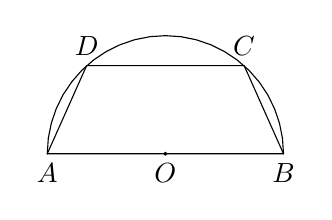
\begin{tikzpicture}[line cap=round,line join=round]
        \draw (-1.5,0.) node[below] {$A$} coordinate (A)
          --(0,0) node[below] {$O$} coordinate (O) circle (.5pt)
          --(1.5,0.) node[below] {$B$} coordinate (B);
        \draw (A)--(-1.,1.12) node[above] {$D$} coordinate (D)
           --(1,1.12) node[above] {$C$} coordinate (C)
           --(B);
        \draw plot[domain=0:pi,variable=\t]
          ({1.5*cos(\t r)},{1.5*sin(\t r)});
      \end{tikzpicture}
      \caption{}\label{fig-190215-2300}
    \end{figure}
  \end{example}

  \beginsolution
    方法一: 
    作 $DE\perp AB$ 于 $E$, 连接 $OD$. 设 $DC=l$, $DE=h$, 则 $AE=R-\frac{l}2$, $OE=\frac{l}2$. 对 $\mathrm{Rt}\triangle ADE$ 和 $\mathrm{Rt}\triangle ODE$, 有
    \[x^2=h^2+\Big(R-\frac{l}2\Big)^2,\quad
      R^2=h^2+\Big(\frac{l}2\Big)^2.\]
    \mymarginpar{\centering
      \begin{tikzpicture}[line cap=round,line join=round]
        \draw (-1.5,0.) node[below] {$A$} coordinate (A)
          --(0,0) node[below] {$O$} coordinate (O) circle (.5pt)
          --(1.5,0.) node[below] {$B$} coordinate (B);
        \draw (A)--(-1.,1.12) node[above] {$D$} coordinate (D)
           --(1,1.12) node[above] {$C$} coordinate (C)
           --(B);
        \draw plot[domain=0.:pi,variable=\t]
          ({1.5*cos(\t r)},{1.5*sin(\t r)});
        \draw[densely dashed] ($(A)!(D)!(O)$) node[below] {$E$} 
          coordinate (E)--(D)--(O);
        \draw \myrtsign{4pt}{O}{E};
      \end{tikzpicture}}
    两式作差, $x^2=-Rl+2R^2$ 即  $l=2R-\frac{x^2}R$, 故 $0<x<\sqrt2R$ 且
    \[y=2x+l+2R=2x-\frac{x^2}R+4R.\]
    
    方法二: 
    作 $DE\perp AB$ 于 $E$, $OF\perp AD$ 于 $F$, 则 $AF=\frac{x}2$. 
    由 $\triangle ADE\backsim\triangle AFO$ 知 $\frac{AE}{AD}=\frac{AF}{AO}$, 即 $AE=\frac{x^2}{2R}$, $DC=2R-2AE=2R-\frac{x^2}R$, 结论同上.
    \mymarginpar{\centering
      \begin{tikzpicture}[line cap=round,line join=round]
        \draw (-1.5,0.) node[below] {$A$} coordinate (A)
          --(0,0) node[below] {$O$} coordinate (O) circle (.5pt)
          --(1.5,0.) node[below] {$B$} coordinate (B);
        \draw (A)--(-1.,1.12) node[above] {$D$} coordinate (D)
           --(1,1.12) node[above] {$C$} coordinate (C)
           --(B);
        \draw plot[domain=0.:pi,variable=\t]
          ({1.5*cos(\t r)},{1.5*sin(\t r)});
        \draw[densely dashed] ($(A)!(D)!(O)$) node[below] {$E$} 
          coordinate (E)--(D) ($(A)!0.5!(D)$) coordinate (F)
          node[left,xshift=-2pt] {$F$}--(O);
        \draw \myrtsign{4pt}{O}{E} \myrtsign{4pt}{A}{F};
      \end{tikzpicture}}
      
    注: 以上结果表明, 当 $x=R$ 时, $y=5R$ 最大, 此时梯形 $ABCD$ 为圆内接正六边形的一半.
  \endsolution
  
  \lianxi
  \begin{exercise}
    (1) 若一次函数 $f(x)$ 满足 $3f(x+1)-2f(x-1)=2x+17$, 求 $f(x)$;

    (2) 已知 $f\Big(\dfrac2{x}+1\Big)= x+3$, 求 $f(x)$ 的解析式.
  \end{exercise}

  \beginsolution
    (1) 设 $f(x)=ax+b$, 等式化为 $ax+5a+b=5x+17$, 则 $a=2$, $b=7$, $f(x)=2x+7$.
    
    (2) 设 $\frac2x+1=t$, 则 $t\neq1$, $x=\frac2{t-1}$, 所以 $f(t)=\frac2{t-1}+3$, 即 $f(x)=\frac2{x-1}+3$, $x\neq 1$.
    
    \varexercise 若函数 $f(x)$ 满足 $3f(x)-2f(-x)=5x+17$, 求 $f(x)$.
    
    把式中 $x$ 换成 $-x$, 则 $3f(-x)-2f(x)=-5x+17$, 与前式联立, 解得 $f(x)=x+17$.
    
    \varexercise 若函数 $f(x)$ 满足 $3f(x)-2f\Big(\frac1x\Big)=5x+17$, 求 $f(x)$.
    
    把式中 $x$ 换成 $\frac1x$, 则 $3f\Big(\frac1x\Big)-2f(x)=\frac5x+17$, 与前式联立, 解得 $f(x)=3x+\frac2x+17$.
  \endsolution
  
  \begin{exercise}
    若等腰三角形的周长是 $20$, 底边长 $y$ 是腰长 $x$ 的函数,
    则 $y$ 关于 $x$ 的函数解析式为\,?
  \end{exercise}

  \beginsolution
    $y+2x=20$, 则 $y=20-2x$, $0<x<10$.
    \mymarginpar{注意运用 ``三角形任意两边之和大于第三边'' 求边长取值范围.}
  \endsolution
  
  \subsubsection{由解析式和图象求定义域}
  \begin{example}
    函数 $f(x)=\dfrac{\sqrt{2x-x^2}}{\lg(2x-1)}+(3-2x)^0$ 的定义域是\,?
  \end{example}

  \beginsolution
    $2x-x^2\geqslant0$, $2x-1>0$ 且  $3-2x\neq 0$, 解得 $x\in\Big(\frac12,\frac32\Big)\cup\Big(\frac32,2\Big]$.
  \endsolution
  
  \lianxi
  \begin{exercise}
    函数 $f(x)=\dfrac{\sqrt{4-x^2}}{\ln(x+2)}$ 的定义域是\,?
  \end{exercise}

  \beginsolution
    $4-x^2\geqslant 0$ 且 $x+1>0$, 解得 $x\in(-1,2]$.
  \endsolution
  
  \begin{exercise}
    已知 $y=f(x)$ 的图象如图~\ref{fig-190414-1125} 所示, 
    那么 $f(x)$ 的定义域为\,?值域为\,?
    \begin{figure}[htb]
    \small
    \centering
    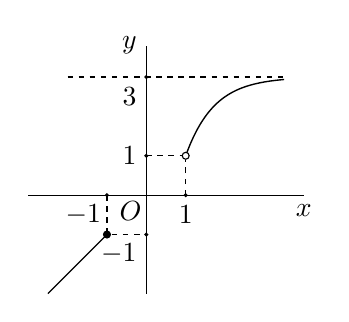
\begin{tikzpicture}[scale=0.5]
      \draw[\myaxisarrow] (-3,0) -- (4,0) node[below] 
        {$x$} coordinate(x axis);
      \draw[\myaxisarrow] (0,-2.5) -- (0,3.8) node[left] 
        {$y$} coordinate(y axis);
      \draw[line width=0.5pt,dash pattern= on 2pt off 2pt] 
        (-2,3)--(3.5,3) (1,0)--(1,0.9) (0,1)--(0.9,1) 
        (-1,0)--(-1,-1)--(0,-1);
      \draw[line width=0.5pt] (-2.5,-2.5)-- (-0.98,-0.98);
      \draw[line width=0.5pt,smooth,samples=100,domain=1.03:3.5] 
        plot(\x,{3-4^(1.5-\x)});
      
      \draw (1,1) circle (2.5pt);
      \draw[fill=black] (1,0.) circle (1pt);
      \draw (1,-0.5) node {$1$};
      \draw[fill=black] (0,1) circle (1pt);
      \draw (0,1) node[left] {$1$};
      \draw[fill=black] (0,-1) circle (1pt) (-1,-1) circle (2.5pt);
      \draw (0,-1.5) node[left] {$-1$};
      \draw[fill=black] (-1,0) circle (1pt);
      \draw (-1.6,-0.5) node {$-1$};
      \draw[fill=black] (0,3) circle (1pt);
      \draw (0,2.5) node[left] {$3$};
      \draw (-0.4,-0.4) node {$O$};
    \end{tikzpicture}
    \caption{}\label{fig-190414-1125}
    \end{figure}
  \end{exercise}

  \beginsolution
    由图, 定义域为 $(-\infty,-1]\cup(1,+\infty)$, 值域为 $(-\infty,-1]\cup(1,3)$.
  \endsolution
  
  \subsubsection{求函数的值域}
  \begin{example}
    求下列函数的值域:
    
    (1) $y=3x^2-x+2$, $x\in [1,3]$;\qquad
    (2) $y=\dfrac{3x+1}{x-2}$.
  \end{example}

  \beginsolution
    (1) 对称轴 $x=-\frac{-1}{2\cdot3}=\frac16$, 则 $y_{\max}=26$, $y_{\min}=4$, 值域 $[4,26]$.
    
    (2) $y=3+\frac7{x-2}$, 则 $y\in(-\infty,3)\cup(3,+\infty)$.
  \endsolution
  
  \subsubsection{分段函数}
  \begin{example}
    已知 $f(x)=\begin{cases}
      2x, & x>0,\\
      f(x+1), & x\leqslant 0,
    \end{cases}$ 那么 $f\Bigl(-\frac43\Bigr)=$\,? 试作出其图象.
  \end{example}

  \beginsolution
    $f\Bigl(-\frac43\Bigr)=f\Bigl(-\frac13\Bigr)= f\Bigl(\frac23\Bigr)= \frac43$. 图象如右图.
    \mymarginpar{\centering
      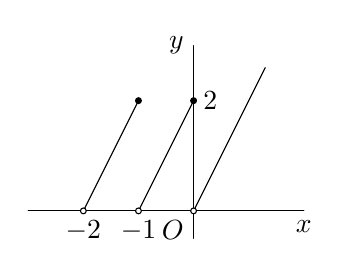
\begin{tikzpicture}[line cap=round,line join=round,scale=0.7]
        \draw[\myaxisarrow] (-3,0) -- (2,0) node[below] {$x$};
        \draw[\myaxisarrow] (0,-0.5) -- (0,3) node[left] {$y$};
        \draw[fill=black] (0,0)--(1.3,2.6) 
          (-1,0)--(0,2) node[right] {$2$} circle (1.5pt) (-2,0)
          --(-1,2) circle (1.5pt);
        \draw[fill=white] (0,0) node[anchor= north east] {$O$} circle (1.5pt) (-1,0) node[below] {$-1$} circle (1.5pt) 
          (-2,0) node[below] {$-2$}  circle (1.5pt);
      \end{tikzpicture}}
  \endsolution
  
  \subsubsection{课堂评价}

  \begin{exercise}
    下列各组函数中, 表示相同函数的有 $\underline{\qquad}$ 组.

    (1) $f(x)=\sqrt{1-x^2}$, $g(x)=1-|x|$, $x\in [-1,1]$;

    (2) $f(x)= \sqrt{x+1}\cdot\sqrt{x-1}$, $g(x)=\sqrt{x^2-1}$.
  \end{exercise}

  \beginsolution
    (1) 由 $f\Big(\frac12\Big)= \frac{\sqrt3}2$, $g\Big(\frac12\Big)= \frac12$ 知 $f(x)\neq g(x)$. 图象如右图.
    \mymarginpar{\centering
      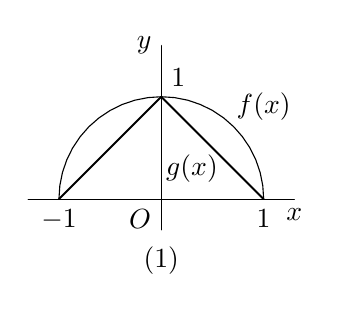
\begin{tikzpicture}[line cap=round,line join=round,scale=1.3]
        \draw[\myaxisarrow] (-1.3,0) -- (1.3,0) node[below] {$x$};
        \draw[\myaxisarrow] (0,-0.3) -- (0,1.5) node[left] {$y$};
        \draw[line width=0.7pt] (0,0) node[anchor= north east] {$O$} 
          (-1,0) node[below] {$-1$} --(0,1) node[anchor=south west] {$1$} --(1,0) node[below] {$1$};
        \draw[line width=0.4pt,variable=\t,domain=0:pi] plot({cos(\t r)},{sin(\t r)});
        \draw (0.3,0.3) node {$g(x)$} (1,0.9) node {$f(x)$} (0,-0.6) node {(1)};
      \end{tikzpicture}}
    
    
    (2) $f(x)$ 定义域为 $[1,+\infty)$, $g(x)$ 定义域为 $(-\infty,-1]\cup [1,+\infty)$, 故 $f(x)\neq g(x)$. 图象如右图.
    \mymarginpar{\centering
      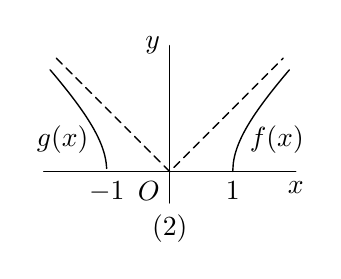
\begin{tikzpicture}[line cap=round,line join=round,scale=0.8]
        \draw[\myaxisarrow] (-2,0) -- (2,0) node[below] {$x$};
        \draw[\myaxisarrow] (0,-0.5) -- (0,2) node[left] {$y$};
        \draw[line width=0.5pt,densely dashed] (-1.8,1.8)--(0,0) node[anchor= north east] {$O$} --(1.8,1.8);
        \draw[line width=0.5pt,samples=100,smooth] 
        plot[domain=-1.9:-1](\x,{sqrt((\x)^2-1)}) 
        plot[domain=1:1.9](\x,{sqrt((\x)^2-1)});
        \draw (-1.7,0.5) node {$g(x)$} (1.7,0.5) node {$f(x)$} (0,-0.9) node {(2)} (-1,0) node[below] {$-1$} (1,0) node[below] {$1$};
      \end{tikzpicture}}
    
    综上知, 填 ``$0$''.
  \endsolution
  
  \begin{exercise}
    已知函数 $f(x)=\sqrt{x-1}$. 若 $f(a)=3$, 则实数 $a=$\,?
  \end{exercise}

  \beginsolution
    $\sqrt{a-1}=3$, $a=10$.
  \endsolution
  
  \begin{exercise}
    函数 $y=\dfrac{x-3}{\sqrt{x+2}}-\sqrt{1-x}$ 的自变量 $x$ 的取值范围是\,?
  \end{exercise}

  \beginsolution
    $x+2>0$ 且 $1-x\geqslant 0$, 则 $x\in(-2,1]$.
  \endsolution
  
  \begin{exercise}
    函数 $f(x)= \sqrt{1-2^x}+ \dfrac1{\sqrt{x+3}}$ 的定义域为\,? 值域为\,?
  \end{exercise}

  \beginsolution
    $1-2^x\geqslant 0$ 且 $x+3>0$, 则 $x\in(-3,0]$. 由 $f(x)$ 单减知值域为 $\Big[1+\frac{\sqrt3}3,+\infty\Big)$.
  \endsolution
  
  \subsection{课后练习}
  
  \begin{exercise}
    已知函数 $f(x)=\dfrac{x+a}{x-6}$ 过点~$P(2,-1)$, 那么 $f(1)=$\,?
  \end{exercise}

  \beginsolution
    $\frac{2+a}{2-6}=-1$, 则 $a=2$, $f(1)=-\frac35$.
  \endsolution
  
  \begin{exercise}
    函数 $f(x)= \sqrt{x} \ln(1-x)$, $g(x)= \dfrac{\ln x}{\sqrt{1-x}}$ 的定义域分别是\,?
  \end{exercise}

  \beginsolution
    对 $f(x)$, $x\geqslant 0$ 且 $1-x>0$, 则 $x\in[0,1)$. 
    对 $g(x)$, $x>0$ 且 $1-x\geqslant0$, 则 $x\in(0,1]$.
  \endsolution
  
  \begin{exercise}
    已知函数 $f(x)=\begin{cases}
      x^2+1, & x\leqslant 1,\\
      -2x^2+x, & x>1,
      \end{cases}$ 那么 $f\big(f(1)\big)=$\,?
  \end{exercise}

  \beginsolution
    $f\big(f(1)\big)=f(2)=-6$.
    
    \varexercise $f(x)$ 同上, 若关于 $x$ 的方程 $f(x)=m$ 有两个解, 求 $m$ 的取值范围.
    
    图解可知, $m\in(1,2]$. 
  \endsolution
  
  \begin{exercise}
    已知函数 $f(x)$ 满足 $f(x+1)=4x-1$, 那么 $f(x)=$\,?
  \end{exercise}

  \beginsolution
    $f(x)=4(x-1)-1=4x-5$.
  \endsolution
  
  \begin{exercise}
    设 $f(x)=\begin{cases}
      x^2+2x+2, & x\leqslant 0,\\
      -x^2, & x>0.
    \end{cases}$ 若 $f\big(f(a)\big)=2$, 则 $a=$\,?
  \end{exercise}

  \beginsolution
    若 $f(x)=2$, 则 $x\leqslant 0$ 且 $x^2+2x+2=0$, 解得 $x=0$ 或 $-2$, 所以 $f(a)=0$ 或 $-2$. 讨论知, $a=\sqrt2$.
  \endsolution
  
  \begin{exercise}
    已知函数 $f(x)=\begin{cases}
      -2x, & x<-1,\\
      2, & -1\leqslant x\leqslant 1,\\
      2x, & x>1.\end{cases}$

    (1) 求 $f\Bigl(-\dfrac32\Bigr)$, $f\Big(\dfrac12\Big)$, 
        $f(4.5)$, $f\Big(f\Big(\dfrac12\Big)\Big)$;
        
    (2) 若 $f(a)=6$, 求 $a$ 的值;\qquad
    (3) 求 $f(x)$ 的值域.
  \end{exercise}

  \beginsolution
    (1) $f\Bigl(-\dfrac32\Bigr)=3$, $f\Big(\dfrac12\Big)=2$, 
      $f(4.5)=9$, $f\Big(f\Big(\dfrac12\Big)\Big)=f(2)=4$.
      
    (2) 若 $a<-1$, 则 $-2a=6$, $a=-3$. 若 $a>1$, 则 $2a=6$, $a=3$. 综上知, $a=-3$ 或 $3$.
    
    (3) 作图可知, 值域为 $[2,+\infty)$.
  \endsolution
  
%%%%%%%%%%%%%%%%%%%%%%